%%%%%%%%%%%%%%%%%%%%%%%%%%%%%%%%%%%%%%%%%
% Large Colored Title Article
% LaTeX Template
% Version 1.1 (25/11/12)
%
% This template has been downloaded from:
% http://www.LaTeXTemplates.com
%
% Original author:
% Frits Wenneker (http://www.howtotex.com)
%
% License:
% CC BY-NC-SA 3.0 (http://creativecommons.org/licenses/by-nc-sa/3.0/)
%
%%%%%%%%%%%%%%%%%%%%%%%%%%%%%%%%%%%%%%%%%

%-------------------------------------------------------------------------------
%	PACKAGES AND OTHER DOCUMENT CONFIGURATIONS
%-------------------------------------------------------------------------------

% A4 paper and 11pt font size
\documentclass[DIV=calc, fontsize=12pt, twocolumn]{scrartcl}

\usepackage{graphicx}
\usepackage[english]{babel} % English language/hyphenation
\usepackage[protrusion=true,expansion=true]{microtype} % Better typography
\usepackage{amsmath,amsfonts,amsthm} % Math packages
\usepackage[svgnames]{xcolor} % Enabling colors by their 'svgnames'
\usepackage[hang, small,labelfont=bf,up,textfont=it,up]{caption} % Custom captions under/above floats in tables or figures
\usepackage{booktabs} % Horizontal rules in tables
\usepackage{fix-cm}	 % Custom font sizes - used for the initial letter in the document
\usepackage{enumitem}
\usepackage{sectsty} % Enables custom section titles
\allsectionsfont{\usefont{OT1}{phv}{b}{n}} % Change the font of all section commands

\usepackage{fancyhdr} % Needed to define custom headers/footers
\pagestyle{fancy} % Enables the custom headers/footers
\usepackage{lastpage} % Used to determine the number of pages in the document (for "Page X of Total")

% Headers - all currently empty
\lhead{}
\chead{}
\rhead{}

% Footers
\lfoot{}
\cfoot{}
\rfoot{\footnotesize Page \thepage\ of \pageref{LastPage}} % "Page 1 of 2"

\renewcommand{\headrulewidth}{0.0pt} % No header rule
\renewcommand{\footrulewidth}{0.4pt} % Thin footer rule

\usepackage{lettrine} % Package to accentuate the first letter of the text
\newcommand{\initial}[1]{ % Defines the command and style for the first letter
\lettrine[lines=3,lhang=0.3,nindent=0em]{
%\color{DarkGoldenrod}
{\textsf{#1}}}{}}

%----------------------------------------------------------------------------------------
%	TITLE SECTION
%----------------------------------------------------------------------------------------

\usepackage{titling} % Allows custom title configuration

\newcommand{\HorRule}{\color{Black} \rule{\linewidth}{1pt}} % Defines the gold horizontal rule around the title

\pretitle{\vspace{-30pt} \begin{flushleft} \HorRule \fontsize{38}{38} \usefont{OT1}{phv}{b}{n} \color{DarkRed} \selectfont} % Horizontal rule before the title

\title{Baxter Robots are Learning to Think, See, and Cook} % Your article title

\posttitle{\par\end{flushleft}\vskip 0.5em} % Whitespace under the title

\preauthor{\begin{flushleft}\large \lineskip 0.5em \usefont{OT1}{phv}{b}{sl} \color{DarkRed}} % Author font configuration

\author{Benjamin Bengfort, Victoria Cepeda, Huijing Gong, Nicholas Labich, \& Mahmoud Sayed  } % Your name

\postauthor{\footnotesize \usefont{OT1}{phv}{m}{sl} \color{Black} % Configuration for the institution name
University of Maryland, College Park % Your institution

\par\end{flushleft}\HorRule} % Horizontal rule after the title

\date{Thursday, February 26, 2015} % Add a date here if you would like one to appear underneath the title block

%----------------------------------------------------------------------------------------

\begin{document}

\maketitle % Print the title

\thispagestyle{fancy} % Enabling the custom headers/footers for the first page

%----------------------------------------------------------------------------------------
%	ABSTRACT
%----------------------------------------------------------------------------------------

% The first character should be within \initial{}
\initial{B}\textbf{axters are low cost humanoid robots meant for adaptable manufacturing purposes by using long nimble arms and a suite of visual and tactile sensors. At the University of Maryland, researchers are exploring computer vision, machine learning, and artificial intelligence by training the Baxters to pour water into a moving jar, learn to cook by watching YouTube, and work with other robots. }

%----------------------------------------------------------------------------------------
%	ARTICLE CONTENTS
%----------------------------------------------------------------------------------------

\section*{Introduction}

In April 2014, researchers at the University of Maryland acquired two Baxter Intera 3 humanoid robots manufactured by Rethink Robotics \cite{fitzgerald_developing_2013}. Baxter robots are well known for their use in micro-manufacturing as they are specially designed for repeated grasping and moving tasks in a stationary position. While a Baxter's multi-dimensional range of motion is important, what makes them especially interesting is their adaptability. Baxter robots are “trained” – not programmed – on work sites. Human workers move the Baxter’s incredibly flexible robotic arms to “show” Baxter how to do a particular task. This ability, combined with Baxter's powerful onboard processing, a suite of sensors, and smooth operating mechanisms, makes Baxter ideal for research.

% A quote here would be perfect!

\begin{figure}
	\centering
	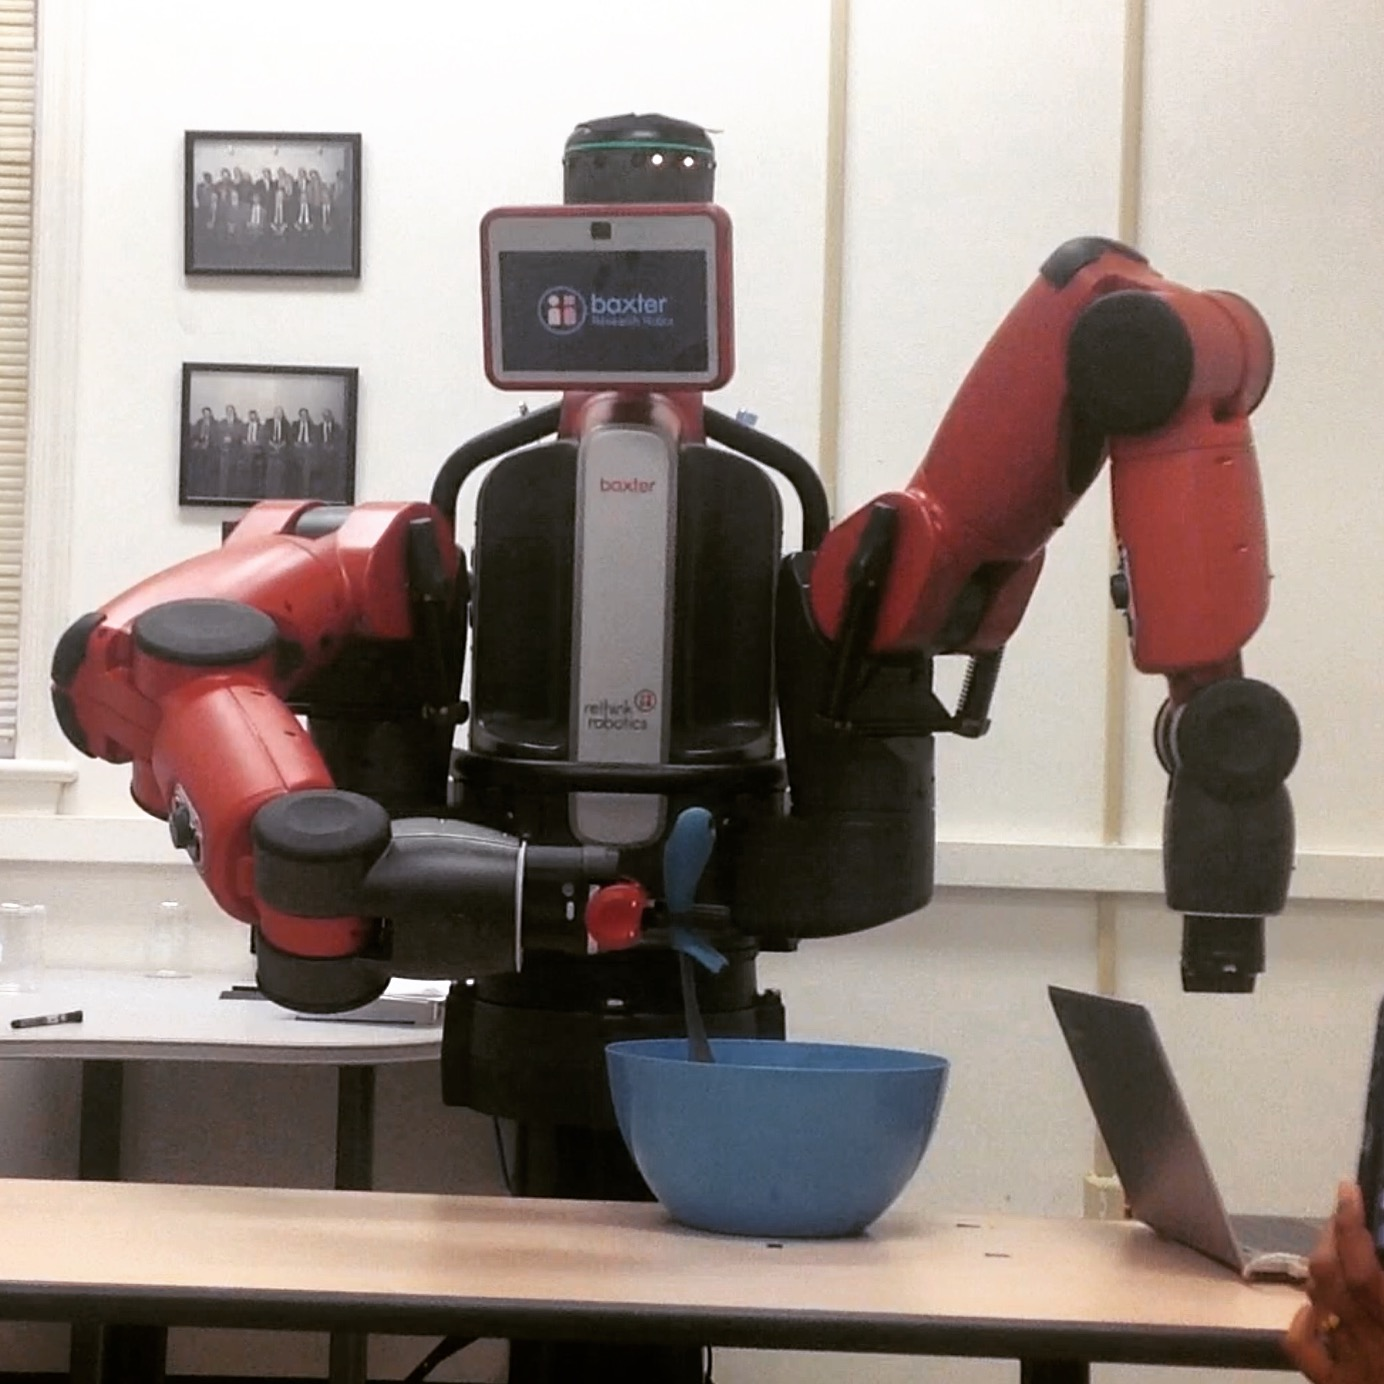
\includegraphics[width=0.40\textwidth]{IMG_0175.jpg}
    \caption{\textsf{Baxter stirs a bowl}}
    \label{fig:stir}
    \vspace{-.35in}
\end{figure}

\begin{figure*}
	\centering
    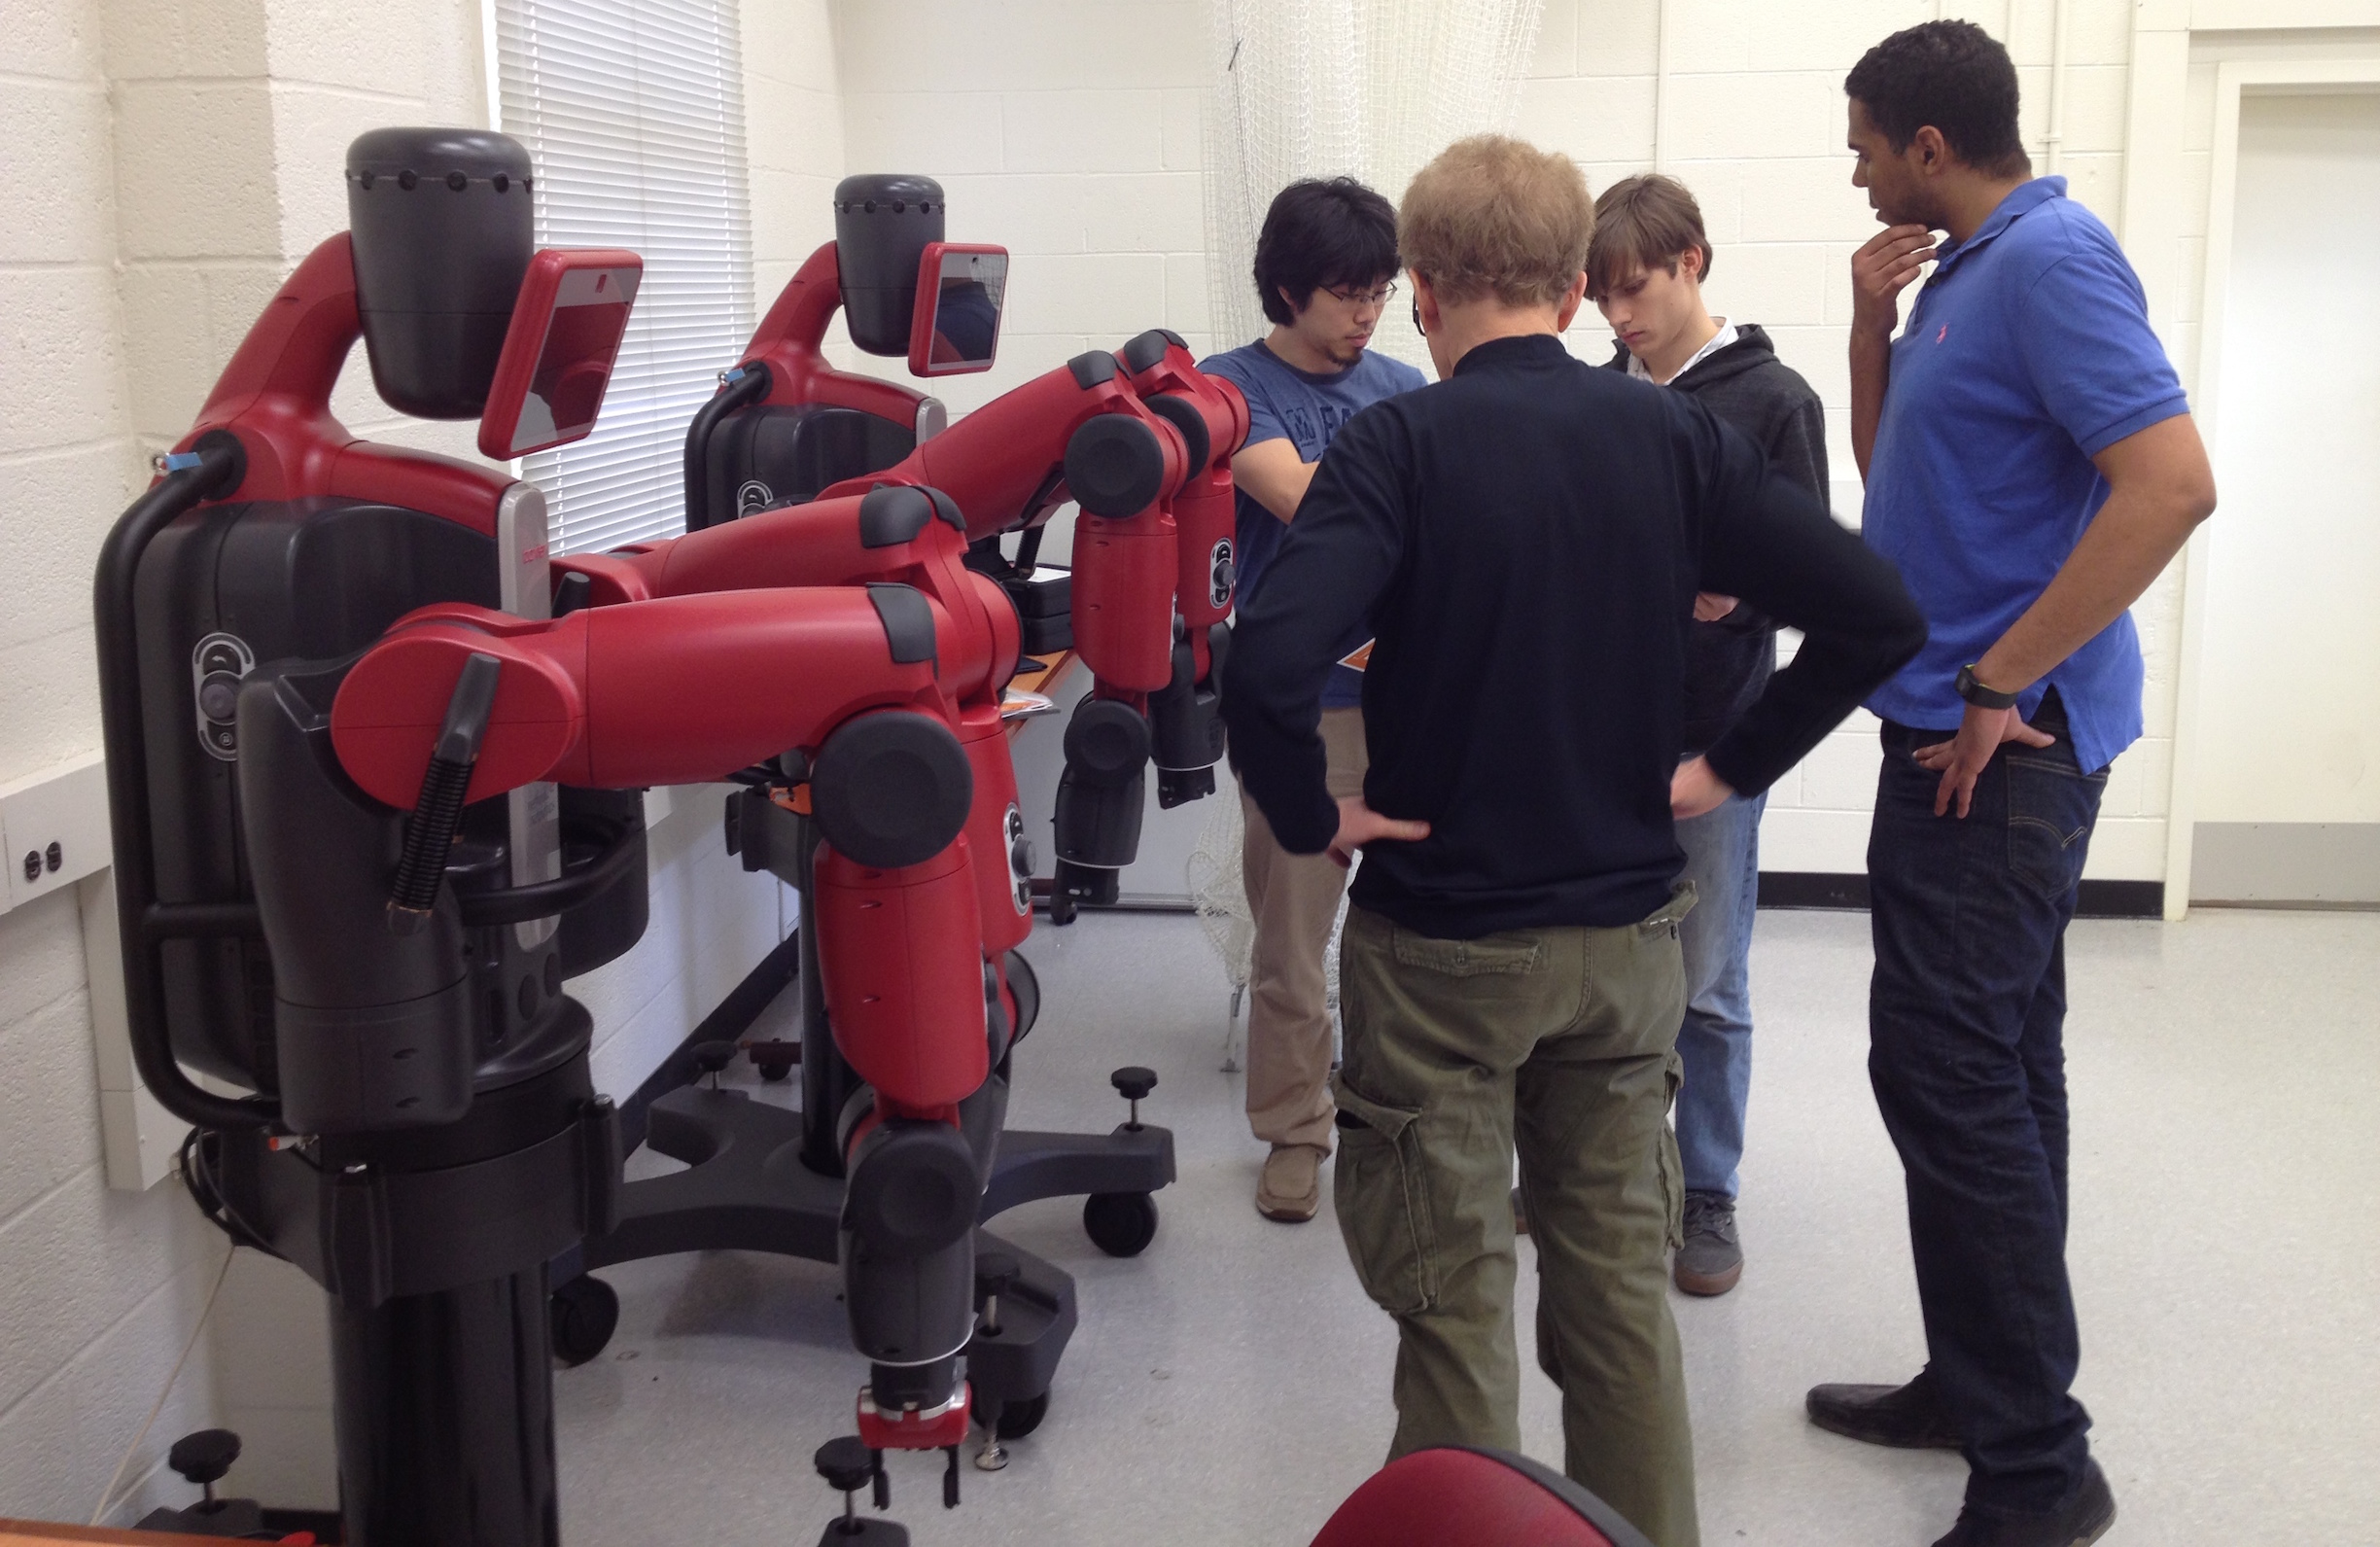
\includegraphics[width=0.90\textwidth]{IMG_1955.jpg}
    \caption{\textsf{UMD researchers apply vision and AI research to practical robots.}}
    \label{fig:robots}
\end{figure*}

In the Computer Science department, research groups have already begun to explore computer vision, machine learning, and artificial intelligence within a robotic context. Three research groups — the Computer Vision Labratory (CFAR), the Metacognitive Lab (MCL), and the Maryland Robotics Center — have been cooperating to produce practical results from their individual theoretical fields. Simple tasks like picking up utensils and stirring bowls, pouring water in a moving container, and building structures from blocks have been quickly achieved thanks to this collaboration. By studying the difficulties involved in teaching Baxter to perform these tasks, the research groups hope to solve larger theoretical challenges.

\section*{Metacognition}

The primary research goal of the Metacognition Lab (MCL) at University of Maryland is to create an enduring artificial agent: one which persists over time, learns from it’s mistakes, interacts with the environment, and constantly acquires new knowledge. An agent of this kind specifically requires metacognition – “thinking about thinking” – to analyze its own cognitive processes and adapt how it thinks to prevent future failures. It primarily does this by attempting to understand anomalies in reasoning, asking itself “what went wrong?”. An enduring agent requires the architectural integration or unification of several components including vision, language processing, reasoning, a knowledge base, goals, and a method of interacting with the world. Using the Baxter platform, the MCL group hopes to put together multi-agent or mixed initiative systems.

Professor Don Perlis and MCL are pursuing more direct artificial intelligence research and using the Baxter as a physical realization of their work. One example is the “Bax’n’Buzz” project, which hopes to create a multi-agent system by pairingd the immobile Baxter with a Parrot AR quadcopter. The quadcopter will be used to extend Baxter’s line of sight and help the Baxter solve problems such as locating a dropped item. The group is also researching mixed-initiative systems that have both a human and the Baxter robot participating in a single scenario. For example, the group is currently exploring a construction domain where a human foreman instructs the Baxter using natural language to build a structure using blocks or other building materials.

\section*{Computer Vision}

Human beings, when learning to cook, may watch others with cooking experience and mimic their actions. With the advent of YouTube and other video-sharing websites, there are significant amounts of training data available; perhaps a robot can learn to cook by watching YouTube videos and mimicking actions. A group led by Professor Yiannis Aloimonos has developed a visual learning system to teach a Baxter robot to cook by watching YouTube \cite{yang_robot_2015}. The team approached the problem from two levels: first, using a low-level visual system which recognizes objects, hands, and types of manipulations from video, and second, a high-level action system which translates the information from the video into actions to be performed by the robot. This system allowed them to use unconstrained YouTube videos as their data source. Much like the push in virtual reality to be able to generate rendered models of real-world environments, the ability to train intelligent systems with real-world sensory input is an important goal for artificial intelligence research.

\section*{Dynamic Pouring}

Professor James Reggia and his group in the Maryland Robotics Center focus on developing imitation learning approaches for motion. In a dynamic fluid pouring task, humans train a Baxter robot to learn by observing errors made by humans and modeling how humans recover from failed action \cite{langsfeld_incorporating_2014}. Using a supervised model of failure-to-success transitions and imitation learning, the group showed that a robot can successfully perform the same task under different variations and conditions without a sophisticated planning system. By restricting a set of task parameters, such as pouring speed, the implementation of their imitation learning approach is able to succeed at this dynamic pouring task.

\begin{figure}
	\centering
	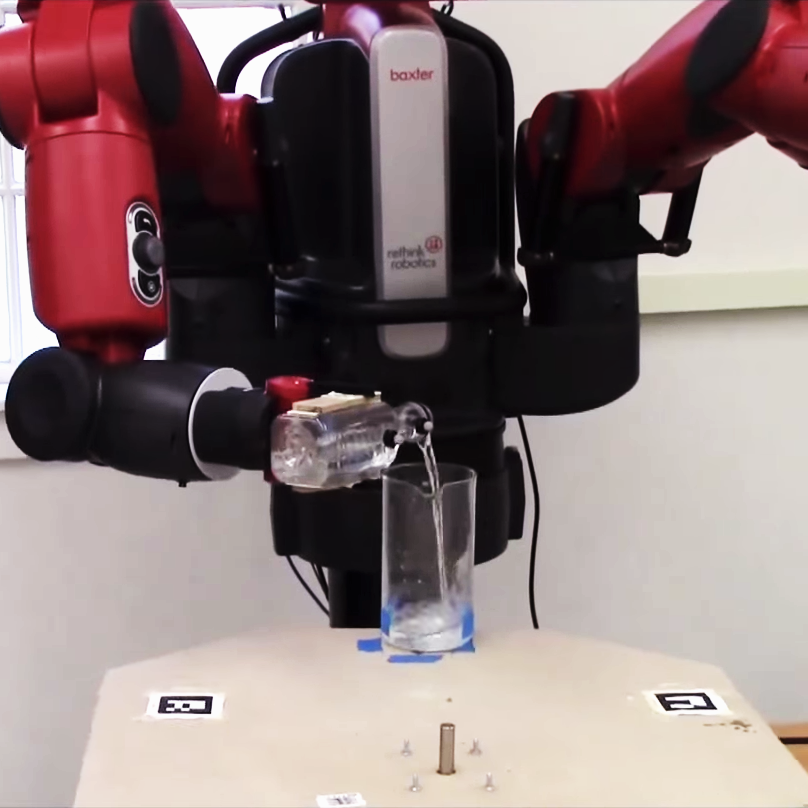
\includegraphics[width=0.40\textwidth]{pour.png}
    \caption{\textsf{Baxter pours water into a moving jar}}
    \label{fig:pour}
    \vspace{-.25in}
\end{figure}

\section*{Conclusion}

The collaboration of vision, robotics, and AI with practical applications using the Baxter robot is allowing research groups to understand visual scenes more thoroughly and to act upon it. The Baxter's unique hardware and programming interface has provided smaller startup costs and reduced the barrier of entry for groups who traditionally don't use robotics platforms in their work. Because of this work, we expect to see robotic behaviors that mimic and learn from humans to do chores or follow directions without external programming. The potential for robots to learn much faster and at a much lower cost, and to share that knowledge with other robots, is a significant step towards developing technologies that could have benefits in areas such as military repair and logistics, smart manufacturing environments, and completely automated warehouses.

For videos showing the Baxter at work, please see: http://ter.ps/8i9 and http://ter.ps/8ia.

%----------------------------------------------------------------------------------------
%	REFERENCE LIST
%----------------------------------------------------------------------------------------


\bibliography{report}
\bibliographystyle{plain}

\subsection*{Contributors}

\begin{itemize}[leftmargin=*,label={},noitemsep]
\item Benjamin Bengfort (bengfort@cs.umd.edu)
\item Huijing Gong (gong@cs.umd.edu)
\item Nicholas Labich (labichn@gmail.com)
\item Mahmoud Sayed (mfayoub@cs.umd.edu)
\item Victoria Cepeda (vickycees@gmail.com)
\end{itemize}

%----------------------------------------------------------------------------------------

\end{document}